\documentclass{beamer} 
\usepackage{amsmath,amsthm}
\usepackage{mathrsfs}
\usepackage{amssymb}
\usepackage[english]{babel}
\usepackage{latexsym}
\usepackage{amsfonts}
\usepackage{graphicx}
\usepackage{float}
\usepackage{graphics}
\usepackage{epsfig}
\usepackage{url}
\usepackage{soul}
\usepackage{listings}
\usepackage{bm}
% \usepackage{minted}


\usetheme{WVU}
\usecolortheme{WVU}
\usepackage{multirow}

\mode<presentation> 

\title[VE401 SU2022 RC week5]{VE401 SU2022 RC week5}

\author[ Shuyu Wu ]{ Shuyu Wu }
\institute[UM-SJTU JI]{UM-SJTU Joint Institute \vspace{.2cm} \\ 
\includegraphics[scale=0.3]{umji_logo.png}\\wushuyu2002@sjtu.edu.cn}
\date[June 2022]{\today}

\begin{document}
\begin{frame} 

\titlepage 

\end{frame} 
\section{Reliability} 
\begin{frame}
       \frametitle{Outline}
       \tableofcontents[currentsection]
\end{frame}

\begin{frame}
    \frametitle{Failure density, Reliability Function}
    Denote $T_A$ to be the random variable indicating that $A$ fails in $T_A$ times. We have
    \[f_A(t)=\lim\limits_{\Delta t\to 0}\frac{P[t\leq T_A\leq t+\Delta t]}{\Delta t}\]
    Actually the failure density $f_A$ is just the PDF of $T_A$. We also denote $F_A$ to be the CDF.\par
    \vspace{0.3cm}
    Reliability function of $T_A$ means the probability that $A$ still survive at time t.
    \[R_{A}(t)=1-F_A(t)\]
    It's called survival function in mathematica or python.
    

\end{frame}

\begin{frame}
    \frametitle{Hazard Rate}
    hazard rate $\rho_A$ is a property that indicates the fail rate at some point given that it's alive before.
    \[\rho_A:=\lim\limits_{\Delta t\to 0}\frac{P[t\leq T_A\leq t+\Delta t|t\leq T_A]}{\Delta t}\]
    It's easy to find that
    \[\rho_A(t)=\frac{f_A(t)}{R_A(t)}\]

\end{frame}

\begin{frame}
    \frametitle{ex 5.1}

    Prove that exponential distribution is the only continuous distribution that has memoryless property.

\end{frame}

\begin{frame}
    \frametitle{ex 5.1 answer}
    Memoryless property implies that $\rho_A=c$, that is,
    \[\frac{F'}{1-F}=c\]
    And we get
    \[F'+cF=c\]
    The initial condition is F(0)=0, and we can get $F=1-e^{-ct}$ and $f(t)=F'(t)=ce^{ct}$, this is an exponential distribution.

\end{frame}

\begin{frame}
    \frametitle{Relationship}
    \[R'(x)=-\rho(x)R(x), R(0)=1\]
    

\end{frame}

\begin{frame}
    \frametitle{Weibull Density}

    The hazard rate of \textbf{Weibull Distribution} is
    \[\rho(t)=\alpha\beta t^{\beta-1}, t,\alpha, \beta>0\]
    It's reliability function is
    \[R(t)=e^{-\alpha t^{\beta}}\]
    The PDF(or failure density) is 
    \[f(t)=\alpha\beta t^{\beta-1}e^{-\alpha t^{\beta}}\]

\end{frame}

\begin{frame}
    \frametitle{Systems in Series and Parallel}

    When A and B are in series, the system fails when any of them fails. Or we can say $S=min\{A,B\}$\par
    $P[S>x]=P[A>x \cap B>x]=P[A>x]P[B>x]$, so $R_{S}=R_{A}R_{B}$ or $F_S=1-(1-F_A)(1-F_B)$\par
    \vspace{0.3cm}
    When A and B are in parallel, the system fails when both of them fails. Or we can say $S=max\{A,B\}$\par
    $P[S<x]=P[A<x \cap B<x]=P[A<x]P[B<x]$, so $F_{S}=F_{A}F_{B}$ or $R_S=1-(1-R_A)(1-R_B)$\par

\end{frame}

\begin{frame}
    \frametitle{End of The Probability Theory}

    That's the end of the probability theory in our course.

\end{frame}

\section{Samples and Data}
\begin{frame}
    \frametitle{Outline}
    \tableofcontents[currentsection]
\end{frame}

\begin{frame}
    \frametitle{What's the difference?}
    \begin{itemize}
        \item Probability: ``Structure" implies ``Property"
        \item Statistics: ``Property" reflects ``Structure". Gain information on the parameters through experiments
    \end{itemize}


\end{frame}

\begin{frame}
    \frametitle{Basic Concepts}
    \textbf{Population:} a large (possibly infinite) collection of targets which we want to calculate probability.\par
    \textbf{A random sample of size n from the distribution of $X$:} a collection of n independent random variables $X_1,...,X_n$, each with the same distribution as $X$.\par
    We say $X_1,\cdots X_n$ are independent, identically distributed (i.i.d.) random sample of $X$. \par
    Sample size usually $\leq 5\%$

\end{frame}

\begin{frame}
    \frametitle{percentiles and quartiles}
    \textbf{(lower)xth percentiles}: The value such that $x\%$ of the data are less or equal to it.\par
    \textbf{quartiles: }$q_1, q_2, q_3$. $IQR=q_3-q_1$
    

\end{frame}

\begin{frame}
    \frametitle{Histograms}

    \textbf{Bins:} the number of categories. Should not be too few or too many.\par
    \textbf{Sturges method}: numbers of bins number k: $k=\lceil \log_{2}{(n)}\rceil+1$. For example, if n=40, k=7.\par
    \textbf{Freedman-Diaconis Rule:} Bin width is $h=\frac{2\cdot IQR}{\sqrt[3]{n}}$\par
    \textbf{Mathematica}: Histogram[Data, {"Raw", "FreedmanDiaconis"}] . Here "Data" is numbers enclosed with big bracket ``\{\}" (Actually, I think this is the very few places that we need mathematica in our course).
\end{frame}

\begin{frame}
    \frametitle{Characteristics of the Data}
    For a set of data $\{x_1, x_2, \dots , x_n\}$, 
    \begin{itemize}
        \item precision : smallest decimal place of the values
        \item sample range: $max\left\{ x_1, x_2,...,x_n \right\}-min\left\{ x_1, x_2,...,x_n \right\}$
        \item bin width: sample range/bin number
        
    \end{itemize}

\end{frame}

\begin{frame}
    \frametitle{Stem-and-Leaf Diagrams}
    See slide P307.\par
    \vspace{0.3cm}
    
    Needs["StatisticalPlots\`{}"]\par
    StemLeafPlot[Floor[Data, 10], IncludeEmptyStems $\rightarrow$ True]

\end{frame}

\begin{frame}
    \frametitle{Boxplots}

    Note: the grade plot on canvas grade is \textbf{not} the Boxplots we teach here.
    \begin{enumerate}
        \item Inner fence: $f_1=q_1-1.5 IQR$, $f_3=q_3+1.5 IQR$
        \item Outer fence: $F_1=q_1-3 IQR$, $F_3=q_3+3 IQR$
        \item The ``whiskers" (lines extending to the left and right of the box) end at the adjacent values (the smallest and biggest sample values in [$f_1,f_3$])
    \end{enumerate}
    See sample exam answer and slide page 310 for reference. Notice that you need to mark solid dots for near outliers, and hollow dots for far outliers.\par
    If the data follow a normal distribution, about 7 out of 1000 samples are near outliers, and there're no far outliers.

\end{frame}

\begin{frame}
    \frametitle{Analysis whether the data follow normal distribution}

    \textbf{Boxplot:} The whiskers are moderately asymmetric but the median line is not too far from the center of the
    box. There is no outlier, and in summary no strong evidence that the data does
    not come from a normal distribution. \par
    \vspace{0.3cm}
    \textbf{Histogram:} This histogram has a unimodal shape which is consistent with a normal distribution. It is not significantly skewed, again consistent with a normal distribution. Therefore, there is no evidence that the data does not come from a normal distribution. 
    
\end{frame}

\section{Parameter Estimation}
\begin{frame}
    \frametitle{Outline}
    \tableofcontents[currentsection]
\end{frame}
\begin{frame}
    \frametitle{Statistics and Estimation}
    \textbf{Statistic:} A random variable that is derived from a random sample $X_1,X_2,...,X_n$ of a population.\par
    Examples:
    \begin{itemize}
        \item quartiles
        \item sample maximum
        \item sample mean $\overline{X}=\frac{1}{n}\sum\limits_{i=1}^n X_i$
        \item sample variance $S^2=\frac{1}{n-1}\sum\limits_{k=1}^n (X_k-\overline{X})^2$
    \end{itemize}
    

\end{frame}

\begin{frame}
    \frametitle{Point Estimate and Estimator}
    Our goal is to use a statistic to estimate a population parameter. Such statistic is called an estimator. The parameters to be estimated is denoted as $\theta$, and the estimator is written as $\hat{\theta}$.\par
    This kind of approach to estimate a parameter is called \textbf{point estimate}.
    Please always bear in mind that $\hat{\theta}$ is a random variable, while $\theta$ is a non-random parameter.\par
    Some criteria of the estimate: Bias and Mean Square Error(MSE).
    \begin{itemize}
        \item Bias: We hope that the expected value of $\hat{\theta}$ is close or equal to $\theta$. We define $\theta-E[\hat{\theta}]$ to be the bias of $\hat{\theta}$.
        \item Mean Square Error(MSE): We hope the variance of $\hat{\theta}$ is small for large sample size. The mean square error is defined as $MSE[\hat{\theta}]:=E[(\hat{\theta}-\theta)^2]$
    \end{itemize}
    

\end{frame}

\begin{frame}
    \frametitle{Estimator}
    Clearly, we have
    \[MSE[\hat{\theta}]=Var[\hat{\theta}]+(bias)^2\]
    This formula is very similar to the parallel axis theorem in physics. 
    \begin{figure}[H]
        \centering
        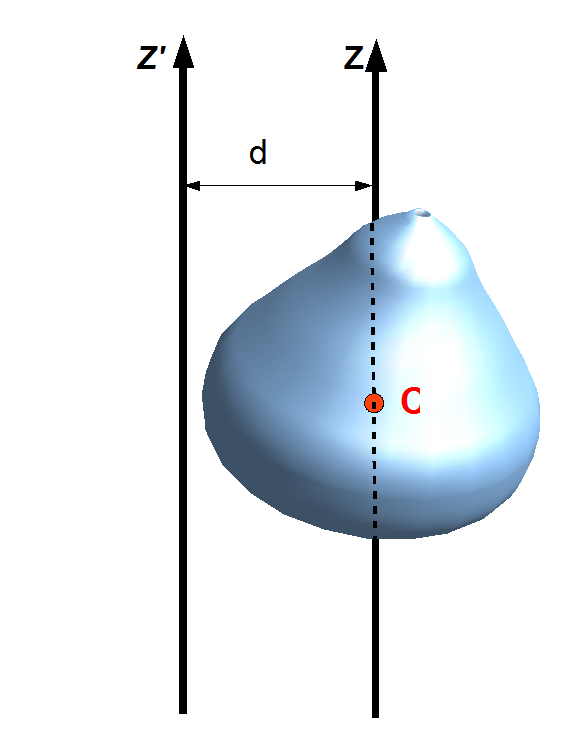
\includegraphics[width=0.17\textwidth,height=0.17\textwidth]{Steiner.png}
        \caption{parallel axis theorem}
    \end{figure}\par
    \[I_{z'}=I_{z}+md^2\]
    The fact is that, you can treat parallel axis theorem as an instance of the MSE formula above. This is the mathematical essence of that physics theorem.
    
\end{frame}

\begin{frame}
    \frametitle{The Mean of the Sample}
    Suppose $E[X]=\mu$, and we have i.i.d sample $X_1,X_2,\dots , X_n$. The mean value $\overline{X}$ is an unbiased estimator for $\mu$. Also $Var[\overline{X}]=\frac{\sigma^2}{n}$ where $\sigma$ is the standard deviation of $X$.
    

\end{frame}

\begin{frame}
    \frametitle{The Method of Moments}
    Above we have already shown that $\overline{X}$ is an unbiased estimator for $E[X]$. It's also true that $\overline{X^k}=\frac{\sum\limits_{i=1}^n X_{i}^k}{n}$ is an unbiased estimator for $E[X^k]$, the kth moment of $X$.\par
    When we want to estimate parameters other than moments, we can express that parameter in terms of moments, and plug in the experimental(estimated) value of moments.
    

\end{frame}

\begin{frame}
    \frametitle{The Method of Moments for Variance}
    \[Var[X]=E[X^2]-E[X]^2\]
    So to estimate variance of $X$ based on the sample $X_1,X_2,\dots , X_n$, we have 
    \[\widehat{Var[X]}=\overline{X^2}-\overline{X}^2=\frac{1}{n}\sum\limits_{k=1}^n (X_k-\overline{X})^2\]
    This is the point estimate value of variance. Notice that it's \textbf{not} nubiased. The MSE is also not minimized.\par
    To get unbiased estimator, you need to divide (n-1). This is called sample variance. To get minimized estimator, you need to divide (n+1) if it's a normal distribution. (You may see that in the assignment)

    

\end{frame}

\begin{frame}
    \frametitle{ex 5.2}
    Suppose $X\sim B(2,p)$. We have sample value $X_1=X_3=1, X_2=2$. Give an estimator for $p$ using the method of moments.

\end{frame}

\begin{frame}
    \frametitle{ex 5.2 answer}
    $E[X]=2p$, $\overline{X}=\frac{4}{3}$, so $2\hat{p}=\frac{4}{3}, \hat{p}=\frac{2}{3}$

\end{frame}

\begin{frame}
    \frametitle{Method of Maximum Likelihood}
    For a random variable $X$ with some unknown parameter $\theta_1, \theta_2, \dots , \theta_n$, suppose the probability density function is $f(x;\theta_1, \theta_2, \dots , \theta_n)$. Also we have a list of sample value $x_1, x_2, \dots , x_k$.\par
    We define the \textbf{likelihood function} $L(\theta_1, \theta_2, \dots , \theta_n)=\prod\limits_{i=1}^{k} f(x_k;\theta_1, \theta_2, \dots , \theta_n)$ , and we want to find the value of $(\theta_1, \theta_2, \dots , \theta_n)$ that maximize the likelihood function. This kind of estimation is called maximum likelihood estimation(MLE) \par
    \vspace{0.3cm}
    Remember, likelihood function indicates the relative likelihood that the sample will occur with the given parameter set. It's not probability. The PDF involved can be either discrete or continuous random variable's.\par
    Also, our target is to find $(\theta_1, \theta_2, \dots , \theta_n)$ that maximize the likelihood function. The maximized value itself is not important. So we tend to take logarithm of the likelihood function.

\end{frame}

\begin{frame}
    \frametitle{ex 5.3}
    Let $X$ be a continuous random variable with density 
    \[f_{X}(x)=\frac{x}{\theta}e^{-\frac{x^2}{2\theta}}(x>0)\]
    and 0 otherwise. Given a series of sample $x_1, x_2, \dots , x_n$, find the maximum likelihood function of $\theta$.
    

\end{frame}

\begin{frame}
    \frametitle{ex 5.3 answer}

    The likelihood function is
    \[L(\theta)=\frac{1}{\theta^n}(\prod\limits_{i=1}^{n}x_i) e^{-\frac{1}{2\theta} \sum\limits_{i=1}^{n}x_{i}^2} \]
    Take logarithm and we get 
    \[\ln L=-n\ln \theta +\ln(\prod\limits_{i=1}^{n}x_i)-\frac{1}{2\theta} \sum\limits_{i=1}^{n}x_{i}^2\]
    Take derivative of $\theta$ and we get
    \[-\frac{n}{\theta}+\frac{1}{2\theta^2}\sum\limits_{i=1}^{n}x_{i}^2=0\]
    And we finally get 
    \[\hat{\theta}=\frac{1}{2n}\sum\limits_{i=1}^{n}x_{i}^2\]

\end{frame}

\begin{frame}
    \frametitle{ex 5.4}
    A kind of LED's life follows an exponential distribution with parameter $\beta$, i.e., $f(x)=\beta e^{-\beta t}(t>0)$. And we have n LED for test.\par
    Normally speaking, after we get the data from these LEDs, we can use MLE to estimate $\beta$. Now, however, we have a limited time/LED, and we can't wait until all the LED reaches the end of their life.\par
    \vspace{0.3cm}
    1. We wait until $m(m<n)$ LED are broken, and we record their lifetime $t_1, t_2, \dots , t_m$. What's the MLE of $\beta$?\par
    \vspace{0.3cm}
    2. We wait until $t_0$, and we find that there're m LED are broken, and we record the broken LED's lifetime $t_1, t_2, \dots , t_m \leq t_0$. What's the MLE of $\beta$?\par

\end{frame}

\begin{frame}
    \frametitle{ex 5.4 answer}
    We've mentioned before that likelihood function is a relative value. It's totally OK to multiply PDF with probability.\par
    1. \par
    The likelihood for the broken m LED are $\beta e^{-\beta t_{i}}, i=1,2,\dots , m$. The likelihood for the other (n-m) LED altogether is $(\int_{t_m}^{+\infty}\beta e^{-\beta t} dt)^{n-m}=e^{-\beta t_m (n-m)}$. So the overall likelihood function is
    \[L=\beta^{m} e^{-\beta [t_1+t_2+\dots +t_m+(n-m) t_m]}\]
    Take logarithm and deviation, we find that $\hat{\beta}=\frac{m}{t_1+t_2+\dots +t_m+(n-m) t_m}$\par
    2.\par
    With the same method we find that
    \[L=\beta^{m} e^{-\beta [t_1+t_2+\dots +t_m+(n-m) t_0]}\]
    And $\hat{\beta}=\frac{m}{t_1+t_2+\dots +t_m+(n-m) t_0}$

\end{frame}

\section{Extra topic and Q\&A}
\begin{frame}
    \frametitle{Outline}
    \tableofcontents[currentsection]
\end{frame}

\begin{frame}
    \frametitle{Shortest Path with direction in DAG}
    DAG: Directed Acyclic Graph
    \begin{figure}[H]
        \centering
        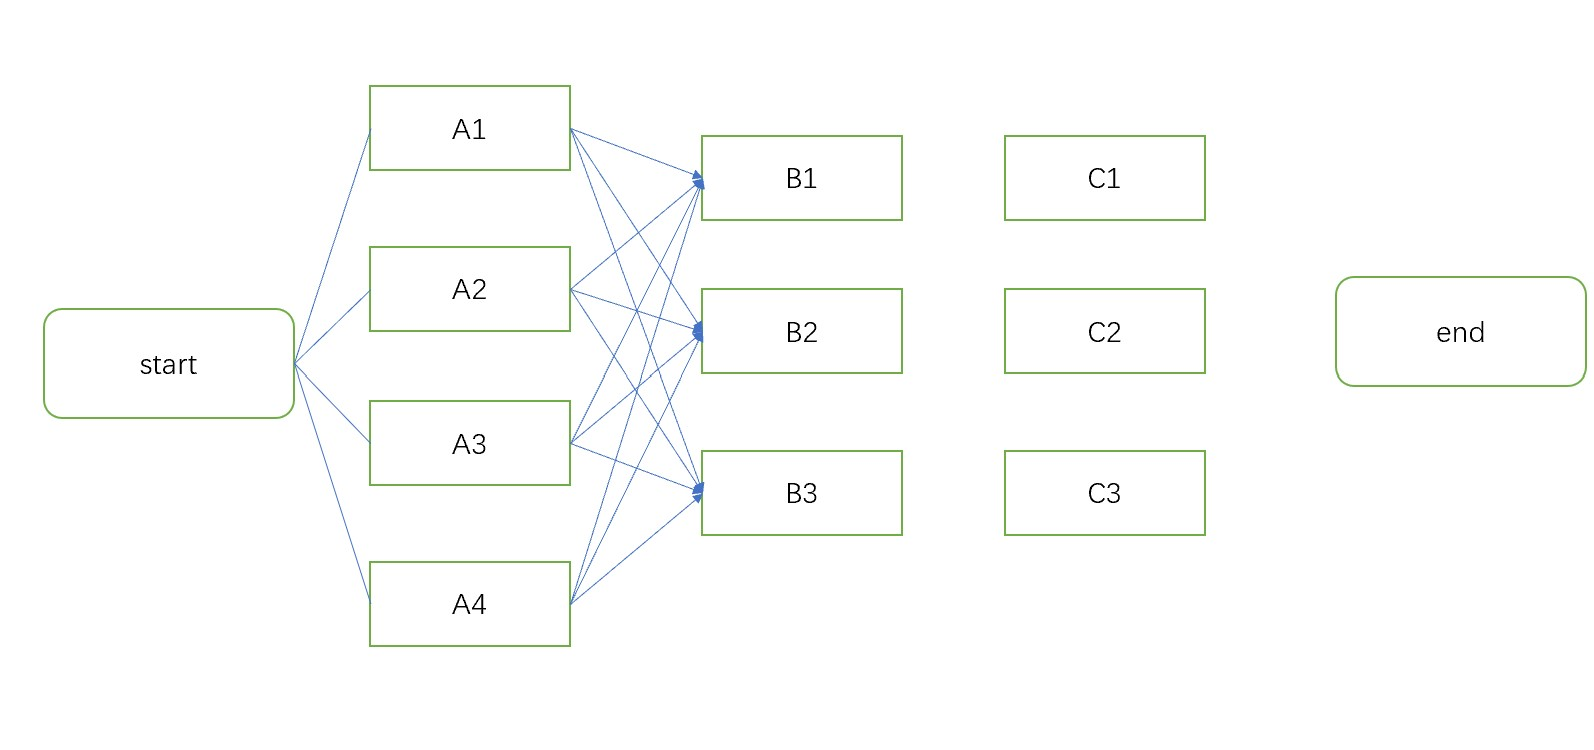
\includegraphics[width=0.55\textwidth,height=0.2\textwidth]{graph1.jpg}
        \caption{Shortest Path with direction}
    \end{figure}\par
    Every path has a weight. How to find the shortest path from Start to End?
    \begin{itemize}
        \item Dijkstra's algorithm: Can't tackle minus weight problem
        \item Viterbi algorithm: Can only deal with DAG, but can tackle minus weight problem, or longest path problem.
    \end{itemize}
    
\end{frame}

\begin{frame}
    \frametitle{Viterbi algorithm}
    \begin{itemize}
        \item It's DP
        \item First find shortest path to $A_1\sim A_4$: straightforward. Record the length on $A_1\sim A_4$.
        \item Next find shortest path to $B_1\sim B_3$: For $B_1$, find the shortest path starting from $A_1\sim A_4$. Record the length. Do the same thing for $B_2$ and $B_3$.
        \item Next find shortest path to $C_1\sim C_3$: For $C_1$, find the shortest path starting from $B_1\sim B_3$. Record the length. Do the same thing for $C_2$ and $C_3$.
        \item Keep doing the same thing until the end of the DAG. Time complexity: $O(LN^2)$($L$ is the step and $N$ is the state)
    \end{itemize}
    

\end{frame}

\begin{frame}
    \frametitle{Application in Probability Theory}
    Stream decoding problem: Take Pinyin as an example. A user input pinyin: $y_1, y_2, \dots , y_n$ and the corresponding Chinese character is $x_1, x_2, \dots , x_n$. Every pinyin correspond to many words, and we make a simplified hypothesis that the process is a Markov process($x_{i+1}$ only depends on $x_{i}$. $x_{i-1}$ and before are not important). Then, each pinyin correspond to a series of Chinese character, which is one step. Each possible Chinese character is one state. And we now want to maximize the multiplication of the weights(the transition probability).\par
    \vspace{0.3cm}
    Viterbi gave up the patent and promote the algorithm. But he still initiate Linkabit company with Irwin Mark Jacobs which sold chips based on this algorithm. Later on, they initiate the famous Qualcomm Inc.

\end{frame}

\begin{frame}
    \frametitle{Extra topic and Q\&A}
    
    Feel free to ask if you have any questions.\par
    The midterm exam is on 22nd, June. Topics include everything before interval estimation.
    
    
\end{frame}

\end{document} 